\documentclass[letterpaper]{article} % DO NOT CHANGE THIS
\usepackage[preprint]{aaai2027}  % DO NOT CHANGE THIS
\usepackage[hyphens]{url}  % DO NOT CHANGE THIS
\usepackage{graphicx} % DO NOT CHANGE THIS
\urlstyle{rm} % DO NOT CHANGE THIS
\def\UrlFont{\rm}  % DO NOT CHANGE THIS
\usepackage{natbib}  % DO NOT CHANGE THIS AND DO NOT ADD ANY OPTIONS TO IT
\usepackage{caption} % DO NOT CHANGE THIS AND DO NOT ADD ANY OPTIONS TO IT
\usepackage{subcaption}
\frenchspacing  % DO NOT CHANGE THIS
\usepackage{booktabs}

% TikZ & Libraries Setup
\usepackage{tikz}
\usetikzlibrary{positioning,arrows.meta,calc,fit,backgrounds}

% Highlighting & Colors Setup
\usepackage{xcolor}

\definecolor{lightbluewash}{RGB}{210, 230, 255}
\definecolor{lightorangewash}{RGB}{255, 220, 185}

% Corrected macro definitions with [1] parameter count explicitly specified
\newcommand{\JJ}[1]{\colorbox{lightbluewash}{\textcolor{blue}{(Jeorge: #1)}}}
\newcommand{\KZ}[1]{\colorbox{lightorangewash}{\textcolor{orange!80!black}{(KZ: #1)}}}

\pdfinfo{
/TemplateVersion (2027.1)
}

\setcounter{secnumdepth}{0}
\title{Bird Transcript: A Web Demonstration of Pronounceable Birdsong Transcription}
\author{
    Jeorge Joshi,
    Kenny Q. Zhu
}
\affiliations{
    University of Texas at Arlington\\
    jxj5621@mavs.uta.edu, kenny.zhu@uta.edu
}

\begin{document}

\maketitle

\begin{abstract}
\JJ{Comments}
\KZ{Comments}
Bird vocalizations lack a standardized, human-readable transcription system.
We demonstrate \textbf{Bird Transcript}, a web application, currently
focused on the canary, that turns an uploaded recording into pronounceable
ASCII tokens: a conv-RNN
locates syllable boundaries, each syllable is assigned to one of 50 acoustic
clusters whose centroids were matched offline, by cosine similarity in a
shared MFCC feature space, to the closest human consonant--vowel unit in the
TIMIT speech corpus, and duration
and pitch contour are encoded inline (e.g.\ \texttt{d\'{\i}iiin}). Users
play back individual syllables, scroll through the synchronized spectrogram
and token sequence, and rotate a 3-D acoustic manifold that plots every
syllable against the reference corpus, seeing a song's structure at a
glance rather than as an opaque list of cluster IDs. The underlying method
achieves an Adjusted Rand Index of 0.64--0.80 against TweetyBERT acoustic
clusters and 69.9\% human token-recognition accuracy against a 20\% chance
baseline, and transfers to a phylogenetically distant species, the Bengalese
finch, without retraining the transcription stage.
\end{abstract}

\begin{links}
    \link{Demo}{https://wp225.github.io/bird-transcript/}
    \link{Code}{https://github.com/wp225/bird-transcript}
\end{links}

\section{Introduction and Motivation}
Ornithologists currently describe bird song with arbitrary integer cluster
IDs \citep{gofman2021tweetybert} or listener-dependent onomatopoeia
\citep{onomatopoeia}, neither of which is interpretable without the
original spectrogram or reproducible across observers. Prior systems either
stop at uninterpretable cluster IDs \citep{gofman2021tweetybert,corvid} or
map vocalizations to phonetic symbols by hand or through an indirect
audio-dataset mapping \citep{ispa,huang2023shibascript}; all run offline and
emit static output that can be read but not heard, compared, or explored.
Human speech, by contrast, is described by a universal phonetic inventory
\citep{arpabet}. We ground bird syllables in that inventory:
each syllable is transcribed with the TIMIT \citep{timit1993}
consonant--vowel unit closest to its acoustic cluster in a shared
26-dimensional MFCC space \citep{davis1980mfcc}, producing a token that is
immediately pronounceable
and legible to a phonetics-aware reader. \textbf{Bird Transcript} makes
that pipeline interactively explorable: a user uploads or selects a
recording and watches it turn into text in real time, rather than reading
numbers off a table in a paper. The current focus species is the canary,
and the Preliminary Evaluation section shows the same pipeline carries over to
a phylogenetically distant species, the Bengalese finch, without retraining
the transcription stage. To our knowledge, this is the first public, playable web
demonstration of a bird-to-human phonetic transcription system.

\section{System Architecture and Technical Approach}
\label{sec:architecture}
Bird Transcript is a FastAPI backend fronted by a single-page,
dependency-free HTML/CSS/JS client (Figure~\ref{fig:architecture}). An
uploaded recording first passes a BirdNET \citep{kahl2021birdnet} species
check that confirms it contains canary vocalization before any transcription
runs, so out-of-domain input is rejected rather than silently
mis-transcribed. Given a verified recording, a ConvRNN segmentor
\citep{das} locates syllable boundaries on the
log-power spectrogram; each syllable clip is split into onset, nucleus, and
offset zones and reduced to a 26-D feature vector (8 MFCCs per zone, plus
voiced fraction \citep{mauch2014pyin} and log-duration). Two consumers read that vector: the syllable is assigned to the nearest of 50
$k$-means centroids, each of which carries a pronounceable token derived
offline by cosine-nearest-neighbour matching against a 62,785-unit TIMIT
reference pool (median centroid similarity 0.843, range 0.765--0.919),
yielding 17 distinct consonant--vowel labels that duration and pitch then
decorate (vowel repetition encodes duration, a diacritic encodes pitch
direction, onset/coda consonants frame the nucleus); and a projection onto the first
three principal components of the same corpus places the syllable on the
acoustic manifold. Because the TIMIT pool and feature extraction are fixed,
the transcription stage needs no per-species retraining --- on the Bengalese
finch \citep{koumura2016} the segmentor, fine-tuned on finch audio, reaches
frame F1 of 97.7\%, and acoustic clusters recover note-type labels at ARI
0.81. The client renders the
spectrogram, token strip, and manifold synchronized to playback and to each
other.

\begin{figure}[t]
\centering
\resizebox{0.88\columnwidth}{!}{%
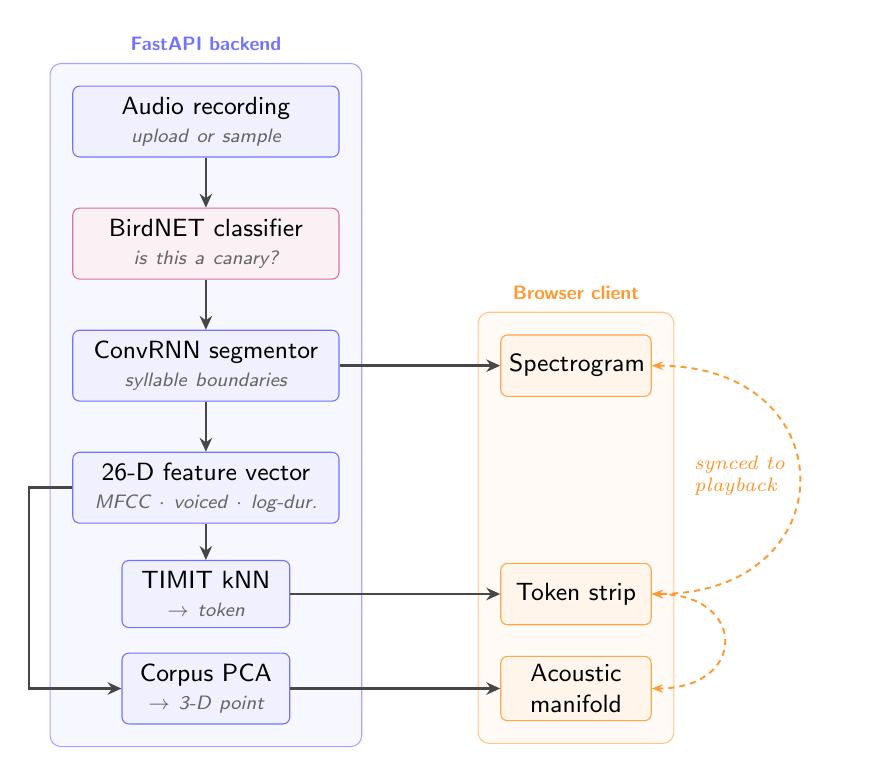
\begin{tikzpicture}[
  every node/.style={font=\small\sffamily},
  box/.style={draw=blue!55, fill=blue!6, rounded corners=2.5pt, align=center,
              minimum height=0.9cm, text width=3.1cm, inner sep=4pt},
  half/.style={box, text width=1.85cm, minimum height=0.78cm},
  gate/.style={draw=purple!55, fill=purple!6, rounded corners=2.5pt, align=center,
               minimum height=0.9cm, text width=3.1cm, inner sep=4pt},
  view/.style={draw=orange!70, fill=orange!8, rounded corners=2.5pt, align=center,
               minimum height=0.78cm, text width=1.7cm, inner sep=3pt},
  arr/.style={-{Stealth[length=5pt,width=4.5pt]}, line width=0.9pt, color=black!72},
  sync/.style={{Stealth[length=4pt]}-{Stealth[length=4pt]}, line width=0.7pt,
               color=orange!80, dashed, dash pattern=on 2.2pt off 1.8pt},
]
% ---- backend column (x = 0), stacked so each output aligns with its view ----
\node[box] at (0, 0)      (audio) {Audio recording\\[-1pt]{\scriptsize\itshape\color{black!60} upload or sample}};
\node[gate] at (0,-1.55)  (birdnet) {BirdNET classifier\\[-1pt]{\scriptsize\itshape\color{black!60} is this a canary?}};
\node[box] at (0,-3.10)   (seg)   {ConvRNN segmentor\\[-1pt]{\scriptsize\itshape\color{black!60} syllable boundaries}};
\node[box] at (0,-4.65)   (feat)  {26-D feature vector\\[-1pt]{\scriptsize\itshape\color{black!60} MFCC $\cdot$ voiced $\cdot$ log-dur.}};
\node[half] at (0,-6.00)  (knn)   {TIMIT kNN\\[-1pt]{\scriptsize\itshape\color{black!60}$\to$ token}};
\node[half] at (0,-7.20)  (pca)   {Corpus PCA\\[-1pt]{\scriptsize\itshape\color{black!60}$\to$ 3-D point}};
\draw[arr] (audio) -- (birdnet);
\draw[arr] (birdnet) -- (seg);
\draw[arr] (seg)   -- (feat);
\draw[arr] (feat.south) -- (knn.north);
% feature vector -> PCA branch, routed down a left channel around the kNN box
\draw[arr] (feat.west) -- ++(-0.55,0) |- (pca.west);
% ---- client column (x = 4.7): views aligned to their sources ----
\node[view] at (4.7,-3.10) (spec)  {Spectrogram};
\node[view] at (4.7,-6.00) (strip) {Token strip};
\node[view] at (4.7,-7.20) (mani)  {Acoustic\\manifold};
% feeds: each horizontal, distinct height -> no crossings
\draw[arr] (seg.east)  -- (spec.west);
\draw[arr] (knn.east)  -- (strip.west);
\draw[arr] (pca.east)  -- (mani.west);
% ---- synchronization among the three views (right side) ----
\draw[sync] (spec.east) to[out=0,in=0,looseness=2.2] (strip.east);
\draw[sync] (strip.east) to[out=0,in=0,looseness=2.6] (mani.east);
\node[font=\scriptsize\itshape, color=orange!85, align=left, text width=1.5cm]
     at (6.95,-4.5) {synced to\\playback};
% ---- panel frames ----
\begin{scope}[on background layer]
  \node[draw=blue!35, fill=blue!3, rounded corners=4pt, inner sep=8pt,
        fit=(audio)(birdnet)(seg)(feat)(knn)(pca)] (bepanel) {};
  \node[draw=orange!45, fill=orange!4, rounded corners=4pt, inner sep=8pt,
        fit=(spec)(strip)(mani)] (clpanel) {};
\end{scope}
\node[font=\scriptsize\sffamily\bfseries, color=blue!55,
      above=1pt of bepanel.north] {FastAPI backend};
\node[font=\scriptsize\sffamily\bfseries, color=orange!80,
      above=1pt of clpanel.north] {Browser client};
\end{tikzpicture}}
\caption{Data flow from an uploaded recording to the three synchronized
views in the client. The hosted build runs this pipeline ahead of time for
a fixed sample library; running the server locally runs it live on any
uploaded audio.}
\label{fig:architecture}
\end{figure}

\paragraph{Deployment.} The hosted demo (a GitHub Pages build) replays a
library of pre-computed canary and Bengalese finch examples, since Pages
serves static files
only and the live model needs a running server; audio upload against the
live model is available by running the same codebase locally. A build script
bakes every bundled recording into static assets, and the deployment
workflow fails closed if the committed client assets or the baked sample set
have drifted from source.

\section{Key Features and User Interface}
\label{sec:features}
Figure~\ref{fig:ui} shows the two synchronized views a user interacts
with.

\begin{figure}[t]
\centering
\begin{subfigure}[b]{\columnwidth}
\centering
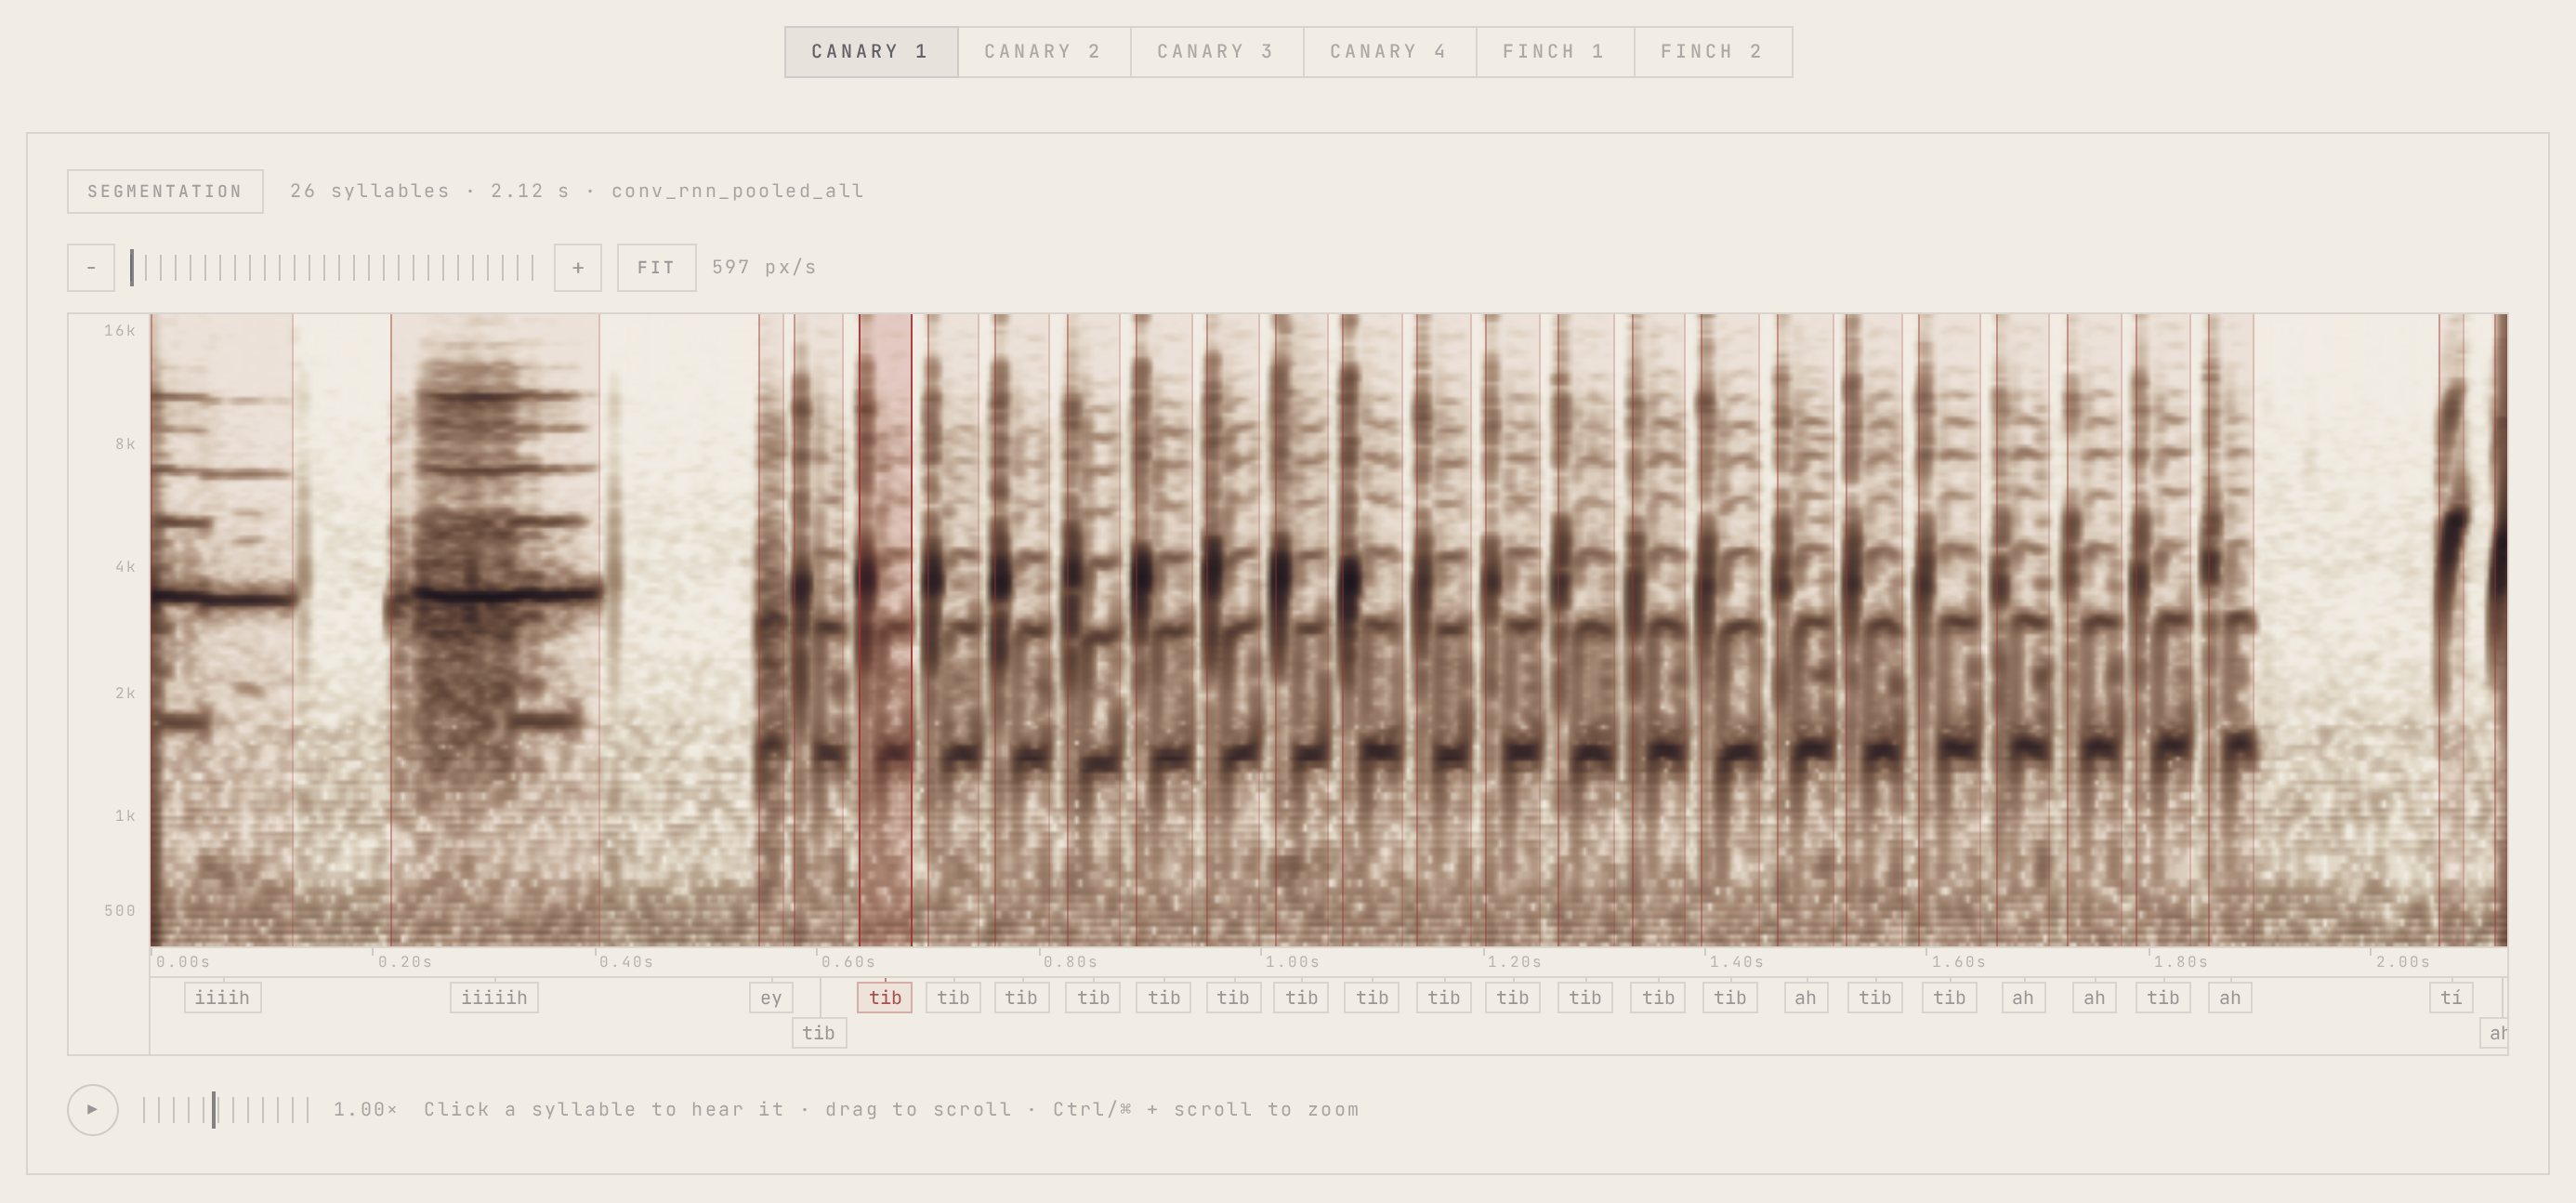
\includegraphics[width=0.72\columnwidth]{figures/ui_transcript.png}
\caption{Sample picker, spectrogram, and token strip for the loaded
recording. Boxed regions mark syllable boundaries; the label beneath each
region is its pronounceable token.}
\label{fig:ui-transcript}
\end{subfigure}
\vspace{4pt}
\begin{subfigure}[b]{\columnwidth}
\centering
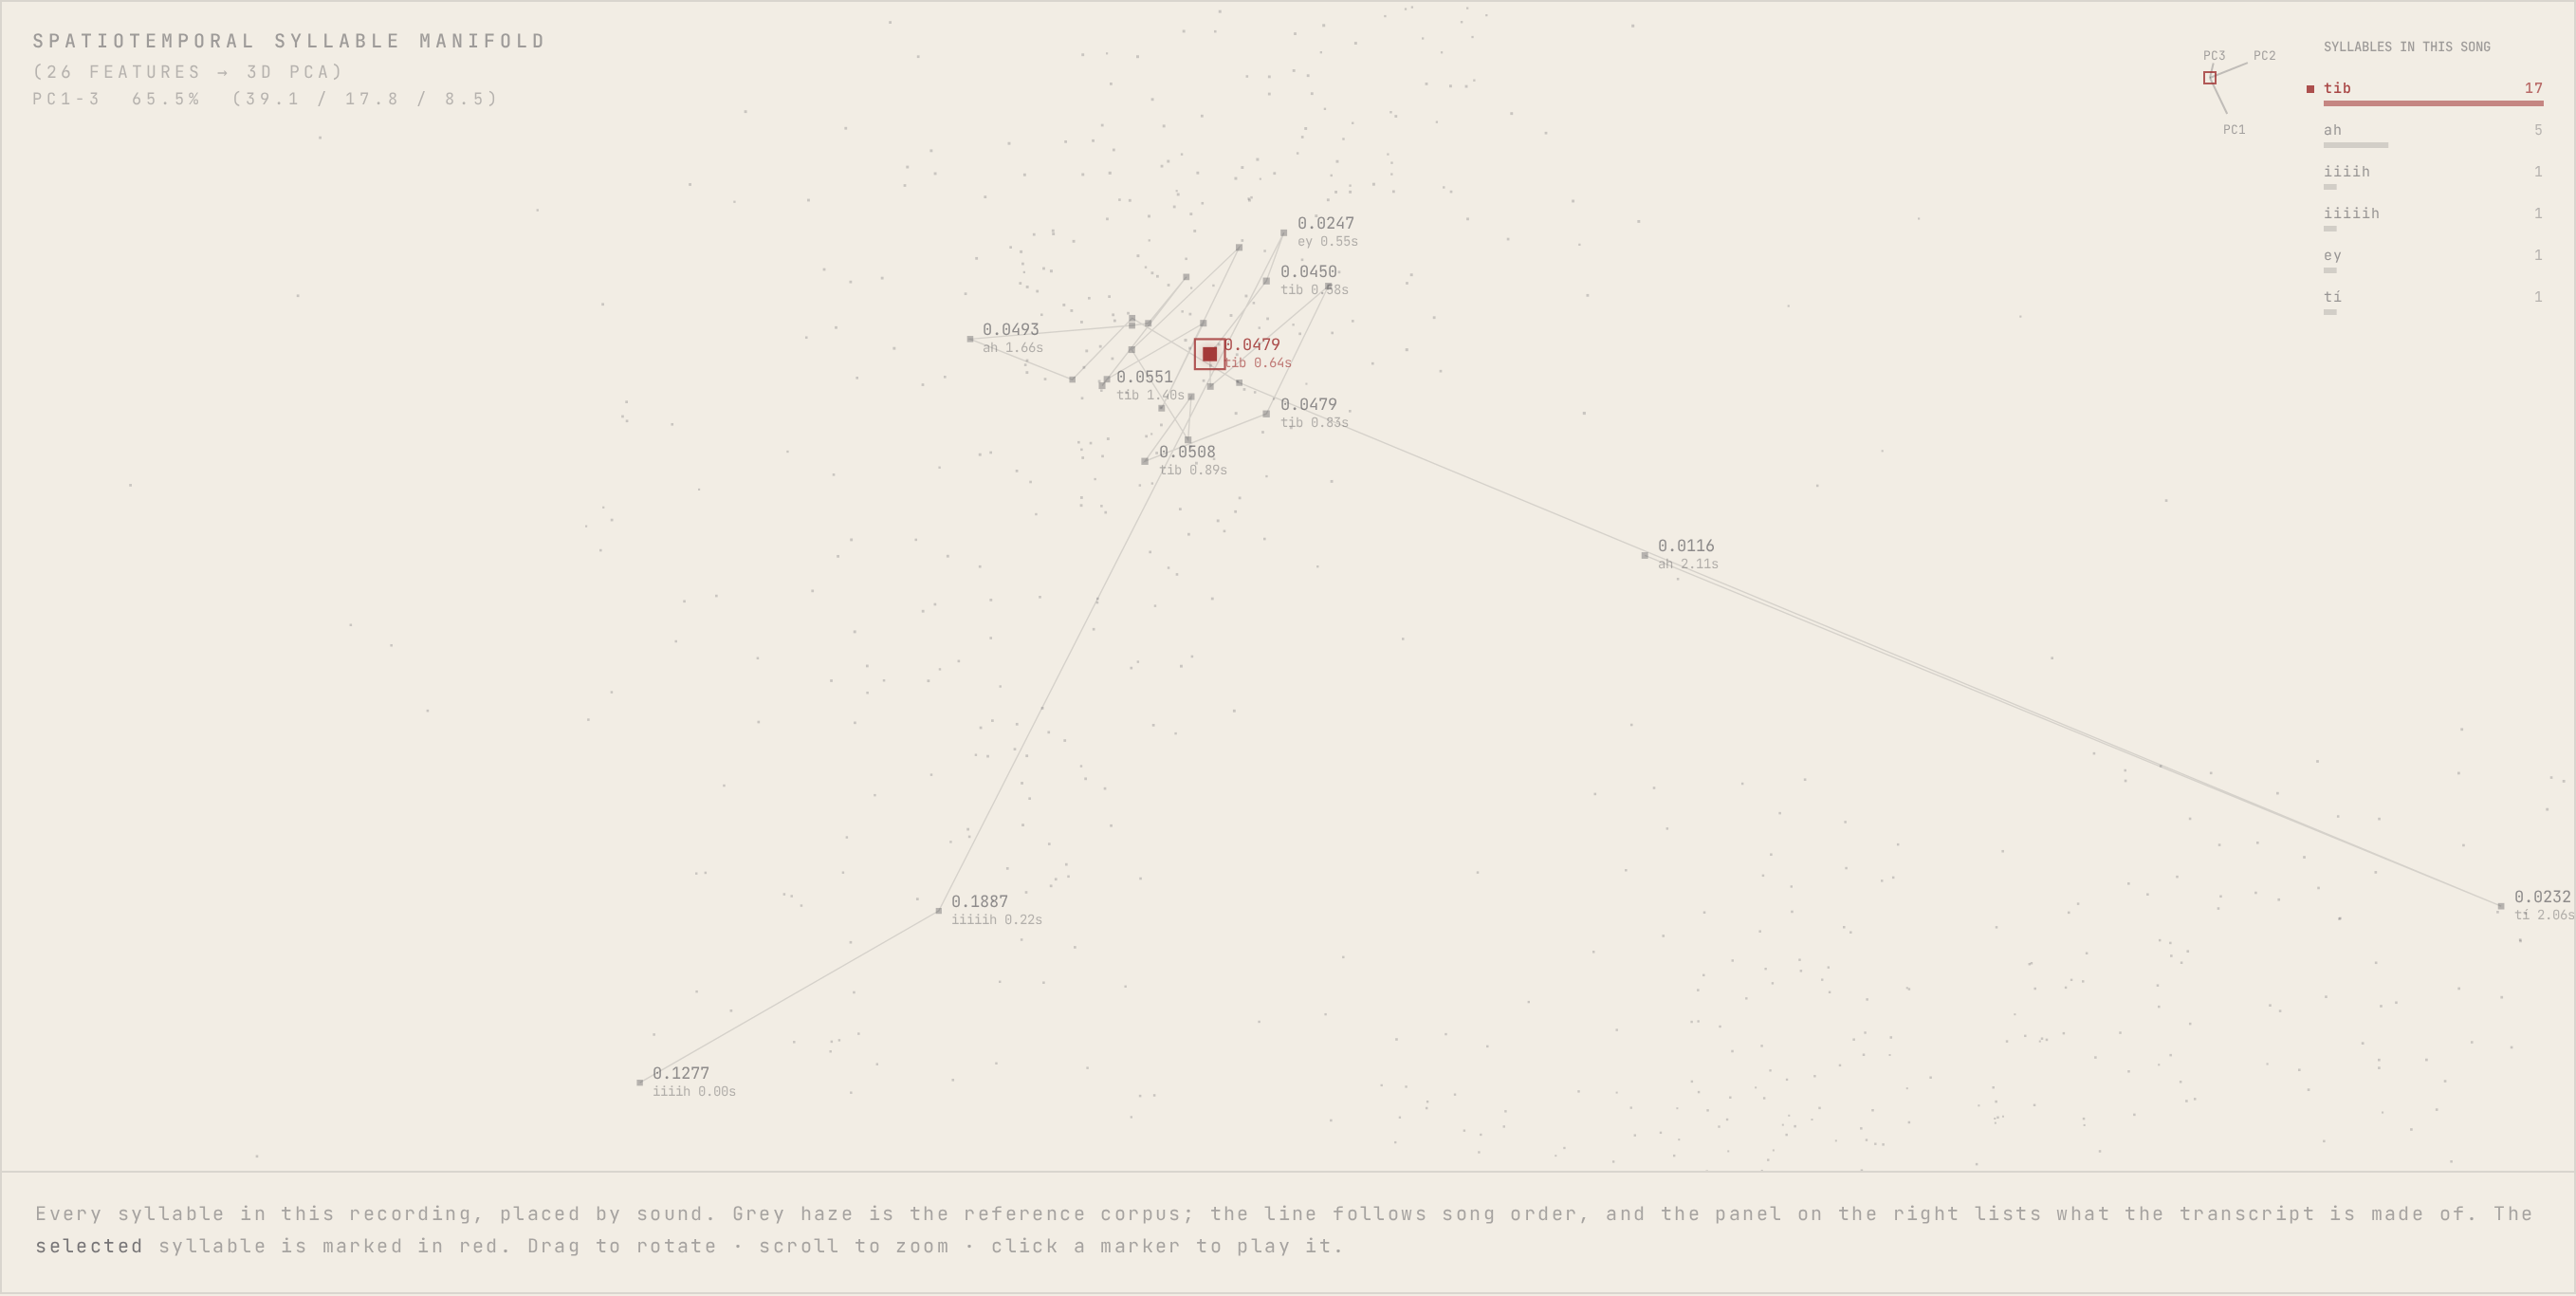
\includegraphics[width=0.72\columnwidth]{figures/ui_manifold.png}
\caption{The same recording's syllables (markers linked in song order, the
selected syllable highlighted) plotted against the reference corpus (grey
haze) on the first three
principal components of the 26-D feature space.}
\label{fig:ui-manifold}
\end{subfigure}
\caption{Bird Transcript's live interface (screenshots from the hosted
demo).}
\label{fig:ui}
\end{figure}

\paragraph{Spectrogram and transcript (Figure~\ref{fig:ui-transcript}).}
Tabs switch between six bundled recordings --- four canary and two Bengalese
finch --- and the spectrogram scrolls beneath its syllable-aligned token
sequence. Clicking a syllable plays its audio in isolation,
\texttt{Ctrl}/\texttt{Cmd}+scroll zooms the time axis, and a speed control
slows playback without desynchronizing the views, so a token can be checked
against what it sounds like rather than taken on trust.

\paragraph{Acoustic manifold (Figure~\ref{fig:ui-manifold}).} Every
syllable in the loaded recording is a point in the 3-D PCA space of the
shared feature manifold, connected in song order, so repeated types
visibly cluster and a phrase becomes a spatial trajectory rather than a
string of IDs. The selected syllable is marked, and a side panel lists the
token types in the recording with their counts. Dragging rotates the view,
scrolling zooms, and clicking a marker plays that syllable, linking the
acoustic-similarity structure behind the tokens directly to sound.

\paragraph{Interaction.} No install is required: the hosted demo runs
entirely in the browser against the bundled sample library described
above. Running the same codebase locally additionally accepts an uploaded
recording and runs the full pipeline --- BirdNET check, segmentation,
transcription, and manifold projection --- on it end to end in seconds, over
the first 30
seconds of the file. Two of the bundled examples are Bengalese finch, a
species not seen during training.

\section{Preliminary Evaluation}
\label{sec:evaluation}
We validate both the pipeline the demo exposes and the demo application
itself, on the public canary corpus of \citet{canary_dataset};
Table~\ref{tab:results} summarizes the numbers quoted in the
abstract. Segmentation F1 under leave-one-bird-out (96.24\%) is the setting
closest to a user uploading a new recording, and at $k{=}50$ the 26-D
$k$-means \citep{lloyd1982} clusters agree with TweetyBERT at ARI 0.64--0.80. Twelve raters
in a forced-choice study recognized isolated tokens at 69.9\% against a
20\% chance baseline ($t(11){=}18.01$, $p{<}0.001$) and rated 71.0\% of
sequences at least 4/5 for intelligibility --- evidence the demo's tokens
are audibly recognizable, not just clusterable.

\begin{table}[t]
\centering
\small
\setlength{\tabcolsep}{4pt}
\renewcommand{\arraystretch}{0.92}
\begin{tabular}{lr}
\toprule
Metric & Value \\
\midrule
Segmentation F1 (pooled) & 98.30\% \\
Segmentation F1 (leave-one-bird-out) & 96.24\% \\
Clustering ARI vs.\ TweetyBERT & 0.64--0.80 \\
Human isolated-token accuracy (chance 20\%) & 69.9\% \\
Sequence intelligibility $\geq$4/5 & 71.0\% \\
Finch zero-shot / fine-tuned segmentation F1 & --- / 97.7\% \\
Finch clustering ARI vs.\ note labels & 0.81 \\
\bottomrule
\end{tabular}
\caption{Validation summary for the pipeline served by the demo.}
\label{tab:results}
\end{table}

\paragraph{Demo application testing.} An automated \texttt{unittest} suite of
18 tests covers both layers: unit tests for the segmentation, feature, and
spectrogram code paths, and browser tests that drive the deployed client ---
sample selection, synchronized playback, zoom, and the manifold. A pre-deploy
check additionally refuses to publish a build whose baked sample set has
drifted from the server's, so a regression surfaces before deployment rather
than in front of a live audience.

\section{Conclusion and Future Work}
Bird Transcript lets a user check the transcription method's central
claim directly, without training data, code, or domain expertise. Because
the transcription stage needs no per-species retraining, any group with a
segmented
recording of an unstudied species can use the same interface for a
comparable transcript. Planned extensions include a rate-limited hosted
inference endpoint, so upload works from the public URL as well as locally,
and a multi-recording manifold view for direct cross-individual and
cross-species comparison.

\bibliography{references}

\end{document}
